\documentclass[table]{beamer}
%[]中可以使用draft、handout、screen、transparency、trancompress、compress等参数

%指定beamer的模式与主题
\mode<presentation>
{
  \usetheme{Madrid}
%\usetheme{Boadilla}
%\usecolortheme{default}
%\usecolortheme{orchid}
%\usecolortheme{whale}
%\usefonttheme{professionalfonts}
}

%\usetheme{Madrid}
%这里还可以选择别的主题:Bergen, Boadilla, Madrid, AnnArbor, CambridgeUS, Pittsburgh, Rochester, Warsaw, ...
%有导航栏的Antibes, JuanLesPins, Montpellier, ...
%有内容的Berkeley, PaloAlto, Goettingen, Marburg, Hannover, ...
%有最小导航栏的Berlin, Ilmenau, Dresden, Darmstadt, Frankfurt, Singapore, Szeged, ...
%有章和节表单的Copenhagen, Luebeck, Malmoe, Warsaw, ...

%\usecolortheme{default}
%设置内部颜色主题(这些主题一般改变block里的颜色);这个主题一般选择动物来命名
%这里还可以选择别的颜色主题,如默认的和有特别目的的颜色主题default,structure,sidebartab,全颜色主题albatross,beetle,crane,dove,fly,seagull,wolverine,beaver

%\usecolortheme{orchid}
%设置外部颜色主题(这些主题一般改变title里的颜色);这个主题一般选择植物来命名
%这里还可以选择别的颜色主题,如默认的和有特别目的的颜色主题lily,orchid,rose

%\usecolortheme{whale}
%设置字体主题;这个主题一般选择海洋动物来命名
%这里还可以选择别的颜色主题,如默认的和有特别目的的颜色主题whale,seahorse,dolphin

%\usefonttheme{professionalfonts}
%类似的还可以定义structurebold,structuresmallcapsserif,professionalfonts


% 控制 beamer 的风格,可以根据自己的爱好修改
%\usepackage{beamerthemesplit} %使用 split 风格
%\usepackage{beamerthemeshadow} %使用 shadow 风格
%\usepackage[width=2cm,dark,tab]{beamerthemesidebar}

%插入音标
\usepackage{tipa}
\AtBeginDocument{
  \renewcommand\textipa{\fontencoding{T3}\selectfont}
}
\AtBeginDocument{
  \renewcommand\textipa[2][r]{{\fontfamily{cm#1}\tipaencoding #2}}
}
\renewenvironment{IPA}[1][r]
 {\fontfamily{cm#1}\tipaencoding}
 {}

% 设定英文字体
%\usepackage{fontspec}
\usepackage[no-math]{fontspec}
\setmainfont{Times New Roman}
\setsansfont{Arial}
\setmonofont{Courier New}

% 设定中文字体
\usepackage[BoldFont,SlantFont,CJKchecksingle,CJKnumber]{xeCJK}
%\setCJKmainfont[BoldFont={Adobe Heiti Std},ItalicFont={Adobe Kaiti Std}]{Adobe Song Std}
\setCJKmainfont[BoldFont={Adobe Heiti Std},ItalicFont={Adobe Kaiti Std}]{WenQuanYi Micro Hei}
\setCJKsansfont{Adobe Heiti Std}
\setCJKmonofont{Adobe Fangsong Std}
\punctstyle{hangmobanjiao}

\defaultfontfeatures{Mapping=tex-text}
\usepackage{xunicode}
\usepackage{xltxtra}

\XeTeXlinebreaklocale "zh"
\XeTeXlinebreakskip = 0pt plus 1pt minus 0.1pt

\usepackage{setspace}
\usepackage{colortbl,xcolor}
\usepackage{hyperref}
%\hypersetup{xetex,bookmarksnumbered=true,bookmarksopen=true,pdfborder=1,breaklinks,colorlinks,linkcolor=blue,filecolor=black,urlcolor=cyan,citecolor=green}
\hypersetup{xetex,bookmarksnumbered=true,bookmarksopen=true,pdfborder=1,breaklinks,colorlinks,linkcolor=cyan,filecolor=black,urlcolor=blue,citecolor=green}

% 插入图片
\usepackage{graphicx}
\graphicspath{{figures/}}
% 图文混排
\usepackage{picins}
\usepackage{floatflt}

% 可能用到的包
\usepackage{amsmath,amssymb}
%插入多媒体
%\usepackage{media9}
%\usepackage{movie15}
\usepackage{multimedia}
\usepackage{multicol}
\usepackage{multirow}

% 定义一些自选的模板,包括背景、图标、导航条和页脚等,修改要慎重
% 设置背景渐变由10%的红变成10%的结构颜色
%\beamertemplateshadingbackground{red!10}{structure!10}
%\beamertemplatesolidbackgroundcolor{white!90!blue}
% 使所有隐藏的文本完全透明、动态,而且动态的范围很小
\beamertemplatetransparentcovereddynamic
% 使itemize环境中变成小球,这是一种视觉效果
\beamertemplateballitem
% 为所有已编号的部分设置一个章节目录,并且编号显示成小球
\beamertemplatenumberedballsectiontoc
% 将每一页的要素的要素名设成加粗字体
\beamertemplateboldpartpage

% item逐步显示时,使已经出现的item、正在显示的item、将要出现的item呈现不同颜色
\def\hilite<#1>{
 \temporal<#1>{\color{gray}}{\color{blue}}
    {\color{blue!25}}
}

\renewcommand{\today}{\number\year 年 \number\month 月 \number\day 日}

%五角星
\usepackage{MnSymbol}

%去除图表标题中的figure等
\usepackage{caption}
\captionsetup{labelformat=empty,labelsep=none}

\usepackage{tabu}
\usepackage{multirow}
%表格自动换行
\usepackage{tabularx} 

% 千分号
%\usepackage{textcomp}

%罗马数字
\makeatletter
\newcommand{\rmnum}[1]{\romannumeral #1}
\newcommand{\Rmnum}[1]{\expandafter\@slowromancap\romannumeral #1@}
\makeatother

%分栏
\usepackage{multicol}

%\usepackage{enumitem}
%\usepackage{enumerate}

%键盘
\usepackage{keystroke}

%插入源代码
\usepackage{listings}
\lstset{
  language=bash,                  % 程序语言名称:TeX, Perl, R, sh, bash, Awk
  basicstyle=\normalsize\tt,      %\tt指monospace字体族,程序源代码使用此族字体表示更加美观
  numbers=left,                   % 行号位置(左侧)
  numberstyle=\small,             % 行号字体的字号
  stepnumber=1,                   % 行号的显示步长
  numbersep=5pt,                  % 行号与代码间距
  backgroundcolor=\color{white},  % 背景色;需要 \usepackage{color}
  showspaces=false,               % 不显示空格
  showstringspaces=false,         % 不显示代码字符串中的空格标记
  showtabs=false,                 % 不显示 TAB
  tabsize=4, 
  frame=shadowbox,                % 把代码用带有阴影的框圈起来
  captionpos=b,                   % 标题位置
  breaklines=true,                % 对过长的代码自动断行
  breakatwhitespace=false,        % 断行只在空格处
  extendedchars=false,            % 解决代码跨页时,章节标题,页眉等汉字不显示的问题
  %escapeinside={\%*}{*},         % 跳脱字符,添加注释,暂时离开 listings 
  %escapeinside=``,
  commentstyle=\color{red!50!green!50!blue!50}\tt,  %浅灰色的注释
  rulesepcolor=\color{red!20!green!20!blue!20},     %代码块边框为淡青色
  keywordstyle=\color{blue!70}\bfseries\tt,         %代码关键字的颜色为蓝色,粗体
  identifierstyle=\tt,
  stringstyle=\tt,                % 代码字符串的特殊格式
  keepspaces=true,
  breakindent=1em,
  %breakindent=22pt,
  %breakindent=4em,
  breakautoindent=true,
  flexiblecolumns=true,
  aboveskip=1em,                  %代码块边框
  xleftmargin=2em,
  xrightmargin=2em
}

%\setbeamercolor{alerted text}{fg=magenta}
\setbeamercolor{bgcolor}{fg=yellow,bg=cyan}
%\setbeamercolor{itemize/enumerate body}{fg=green}

\begin{document}

%\includeonlyframes{current}

\logo{
\includegraphics[height=0.08\textwidth]{tijmu.png}}

% 在每个Section前都会加入的Frame
\AtBeginSection[]
{
  \begin{frame}<beamer>
    %\frametitle{Outline}
    \frametitle{教学提纲}
    \setcounter{tocdepth}{3}
    \begin{multicols}{2}
      \tableofcontents[currentsection,currentsubsection]
      %\tableofcontents[currentsection]
    \end{multicols}
  \end{frame}
}
% 在每个Subsection前都会加入的Frame
\AtBeginSubsection[]
{
  \begin{frame}<beamer>
%%\begin{frame}<handout:0>
%% handout:0 表示只在手稿中出现
    \frametitle{教学提纲}
    \setcounter{tocdepth}{3}
    \begin{multicols}{2}
    \tableofcontents[currentsection,currentsubsection]
    \end{multicols}
%% 显示在目录中加亮的当前章节
  \end{frame}
}

% 为当前幻灯片设置背景
%{
%\usebackgroundtemplate{
%\vbox to \paperheight{\vfil\hbox to
%\paperwidth{\hfil
\includegraphics[width=2in]{tijmu_charcoal.png}\hfil}\vfil}
%}
\begin{frame}[plain]
  \begin{center}
    {\Huge Linux系统概论\\}
    \vspace{1cm}
    {\LARGE 天津医科大学\\}
    %\vspace{0.2cm}
    {\LARGE 生物医学工程与技术学院\\}
    \vspace{1cm}
    {\large 2017-2018学年下学期(春)\\ 2016级生信班}
  \end{center}
\end{frame}
%}



%\includeonlyframes{current}

\title[高级Linux命令]{第五章\quad 高级Linux命令}
\author[Yixf]{伊现富(Yi Xianfu)}
\institute[TIJMU]{天津医科大学(TIJMU)\\ 生物医学工程与技术学院}
\date{2016年3月}


\begin{frame}
  \titlepage
\end{frame}

\begin{frame}[plain,label=current]
  \frametitle{教学提纲}
  \setcounter{tocdepth}{3}
  \begin{multicols}{2}
    \tableofcontents
  \end{multicols}
\end{frame}


\section{引言}
\begin{frame}
  \frametitle{引言}
  \begin{block}{已经学习}
    \begin{itemize}
      \item 命令的工作原理
      \item 常用的基本命令
    \end{itemize}
  \end{block}
  \pause
  \begin{block}{即将学习}
    \begin{itemize}
      \item 正则表达式和元字符
      \item 高级命令:find,grep,sed,AWK
    \end{itemize}
  \end{block}
\end{frame}

\section{正则表达式和元字符}
\begin{frame}
  \frametitle{正则和元字符 | 简介}
  \begin{block}{正则表达式}
    \begin{itemize}
      \item 正则表达式(regular expression)是具有一定句法的集合或短语,表示某类文本或字符串。
      \item 优势:使得用户能够利用比较少的预定义字符集合来表示多种字符组合。
      \item 正则表达式包含元字符或普通字符。
    \end{itemize}
  \end{block}
  \pause
  \begin{block}{元字符}
    \begin{itemize}
      \item 元字符(metacharacter)是代表一组字符或命令的字符。
      \item 优势:减少和命令一起使用的文本数量,用最小的字符集表示多组文本。
    \end{itemize}
  \end{block}
  \pause
  \begin{block}{相关命令}
    less,more; grep,egrep,fgrep; sed,AWK; emacs,vim; \ldots
  \end{block}
\end{frame}

\begin{frame}[fragile]
  \frametitle{Regular Expression | Introduction}
  \textbf{Regular expressions} are text strings used for matching a specific \textbf{pattern}, or to search for a specific location, such as the start or end of a line or a word. Regular expressions can contain both normal characters or so-called \textbf{metacharacters}, such as \verb|*| and \verb|$|.\\
  \vspace{0.3cm}
  Many text editors and utilities such as \textbf{vi}, \textbf{sed}, \textbf{awk}, \textbf{find} and \textbf{grep} work extensively with regular expressions. Some of the popular computer languages that use regular expressions include \textbf{Perl}, \textbf{Python} and \textbf{Ruby}. It can get rather complicated and there are whole books written about regular expressions.\\
  \vspace{0.3cm}
  These regular expressions are different from the wildcards (or "metacharacters") used in filename matching in command shells such as \textbf{bash}.
\end{frame}

\begin{frame}
  \frametitle{Regular Expression | Pattern}
  \begin{figure}
    \centering
    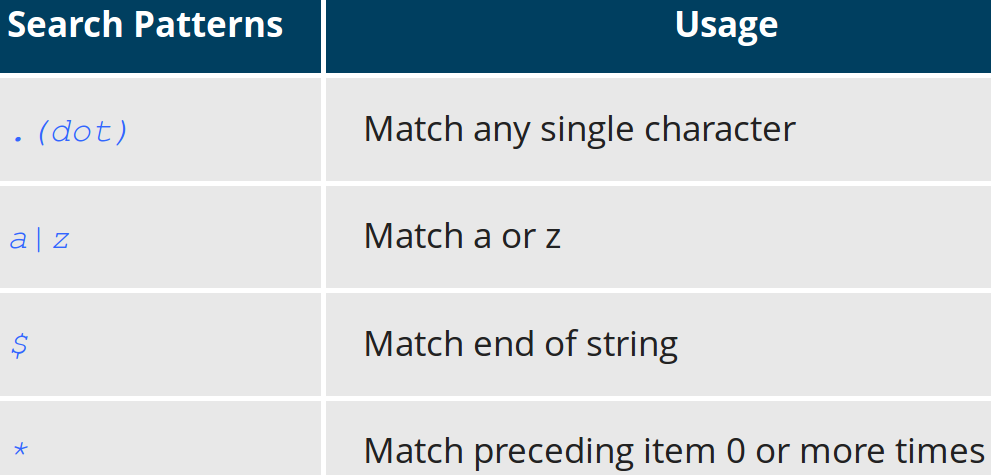
\includegraphics[width=10cm]{c5.re.20.png}
  \end{figure}
\end{frame}

\begin{frame}
  \frametitle{Regular Expression | Example}
  \begin{block}{Sentence}
    the quick brown fox jumped over the lazy dog
  \end{block}
  \begin{figure}
    \centering
    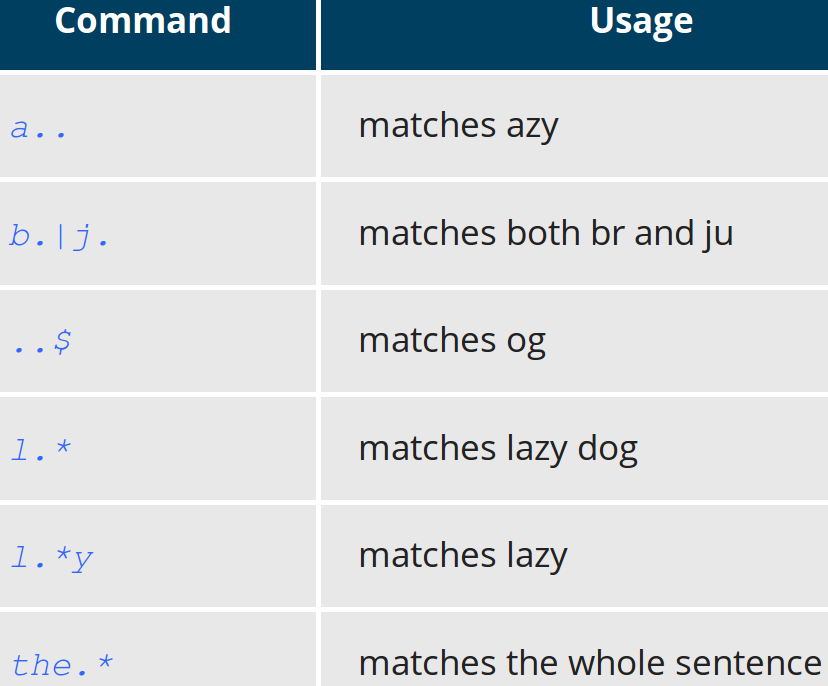
\includegraphics[width=10cm,height=6cm]{c5.re.21.png}
  \end{figure}
\end{frame}

\subsection{元字符}
%\begin{frame}[fragile]
  %\frametitle{正则和元字符 | 元字符}
  %\begin{figure}
    %\centering
    %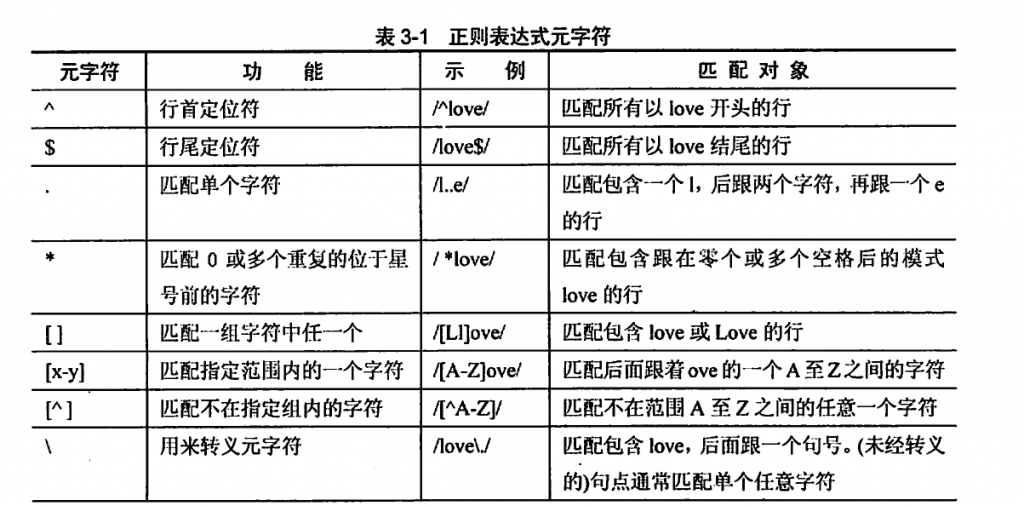
\includegraphics[width=12cm]{c5.meta.01.png}
  %\end{figure}
%\end{frame}

\begin{frame}[fragile]
  \frametitle{正则和元字符 | 元字符 | \alert{字符}}
  \begin{table}
    \centering
    \rowcolors[]{1}{blue!20}{blue!10}
    \begin{tabularx}{\textwidth}{cXll}
      \hline
      \rowcolor{blue!50}元字符 & 功能 & 表达式 & 匹配示例\\
      \hline
      一般字符 & 匹配自身 & \verb|abc| & abc\\
      \verb|.| & 匹配除换行符(\verb|\n|)外的任意一个字符 & \verb|a.c| & abc\\
      \verb|[]| & 匹配字符集中的任意一个字符 & \verb|a[bcd]e| & abe,ace,ade\\
      \verb|[a-z]| & 匹配任意一个小写字母 & \verb|a[a-z]e| & aae,abe,\ldots,aye,aze\\
      \verb|[0-9]| & 匹配任意一个数字 & \verb|a[0-9]e| & a0e,a1e,\ldots,a8e,a9e\\
      \verb|[^]| & 不匹配字符集中的任意一个字符 & \verb|a[^bcd]e| & 除abe,ace,ade外\\
      \verb|\ | & 转义字符(删除紧跟其后的字符的特殊意义) & \verb|a\.c| & \verb|a.c|\\
      \hline
    \end{tabularx}
  \end{table}
\end{frame}

\begin{frame}[fragile]
  \frametitle{正则和元字符 | 元字符 | \alert{字符集}}
  \begin{table}
    \centering
    \rowcolors[]{1}{blue!20}{blue!10}
    \begin{tabularx}{\textwidth}{cXll}
      \hline
      \rowcolor{blue!50}元字符 & 功能 & 表达式 & 匹配示例\\
      \hline
      \verb|\d| & 数字,\verb|[0-9]| & \verb|a\dc| & \verb|a1c|\\
      \verb|\D| & 非数字,\verb|[|\verb|^\d|\verb|]| & \verb|a\Dc| & \verb|abc|\\
      \verb|\s| & 空白字符,\verb|[ \t|\verb|\r|\verb|\n|\verb|\f|\verb|\v|\verb|]| & \verb|a\sc| & \verb|a c|\\
      \verb|\S| & 非空白字符,\verb|[|\verb|^\s|\verb|]| & \verb|a\Sc| & \verb|abc|\\
      \verb|\w| & 单词字符,\verb|[A-Za-z0-9_]| & \verb|a\wc| & \verb|abc|\\
      \verb|\W| & 非单词字符,\verb|[|\verb|^\w|\verb|]| & \verb|a\Wc| & \verb|a c|\\
      \hline
    \end{tabularx}
  \end{table}
\end{frame}

\begin{frame}[fragile]
  \frametitle{正则和元字符 | 元字符 | \alert{量词}}
  \begin{table}
    \centering
    \rowcolors[]{1}{blue!20}{blue!10}
    \begin{tabularx}{\textwidth}{cXll}
      \hline
      \rowcolor{blue!50}元字符 & 功能 & 表达式 & 匹配示例\\
      \hline
      \verb|?| & 匹配前一个字符零次或一次 & \verb|abc?| & ab,abc\\
      \verb|*| & 匹配前一个字符零次或多次 & \verb|abc*| & ab,abccc\\
      \verb|+| & 匹配前一个字符一次或多次 & \verb|abc+| & abc,abccc\\
      \verb|{m}| & 匹配前一个字符m次 & \verb|ab{2}c| & abbc\\
      \verb|{m,n}| & 匹配前一个字符m至n次 & \verb|ab{1,2}c| & abc,abbc\\
      \hline
    \end{tabularx}
  \end{table}
\end{frame}

\begin{frame}[fragile]
  \frametitle{正则和元字符 | 元字符 | \alert{边界}}
  \begin{table}
    \centering
    \rowcolors[]{1}{blue!20}{blue!10}
    \begin{tabularx}{\textwidth}{cXll}
      \hline
      \rowcolor{blue!50}元字符 & 功能 & 表达式 & 匹配示例\\
      \hline
      \verb|^| & 匹配字符串开头 & \verb|^abc| & [开头]abc\\
      \verb|$| & 匹配字符串末尾 & \verb|abc$| & abc[末尾]\\
      \hline
    \end{tabularx}
  \end{table}
\end{frame}

\begin{frame}[fragile]
  \frametitle{正则和元字符 | 元字符 | \alert{其他}}
  \begin{table}
    \centering
    \rowcolors[]{1}{blue!20}{blue!10}
    \begin{tabularx}{\textwidth}{cXll}
      \hline
      \rowcolor{blue!50}元字符 & 功能 & 表达式 & 匹配示例\\
      \hline
      \verb|()| & 分组,创建用于匹配的子串 & \verb|ab(cd)?| & ab,abcd\\
      \verb=|= & 或,两边的项目二选一 & \verb=ab(cd|ef)= & abcd,abef\\
      \hline
    \end{tabularx}
  \end{table}
\end{frame}

\begin{frame}
  \frametitle{正则和元字符 | 元字符}
  \begin{figure}
    \centering
    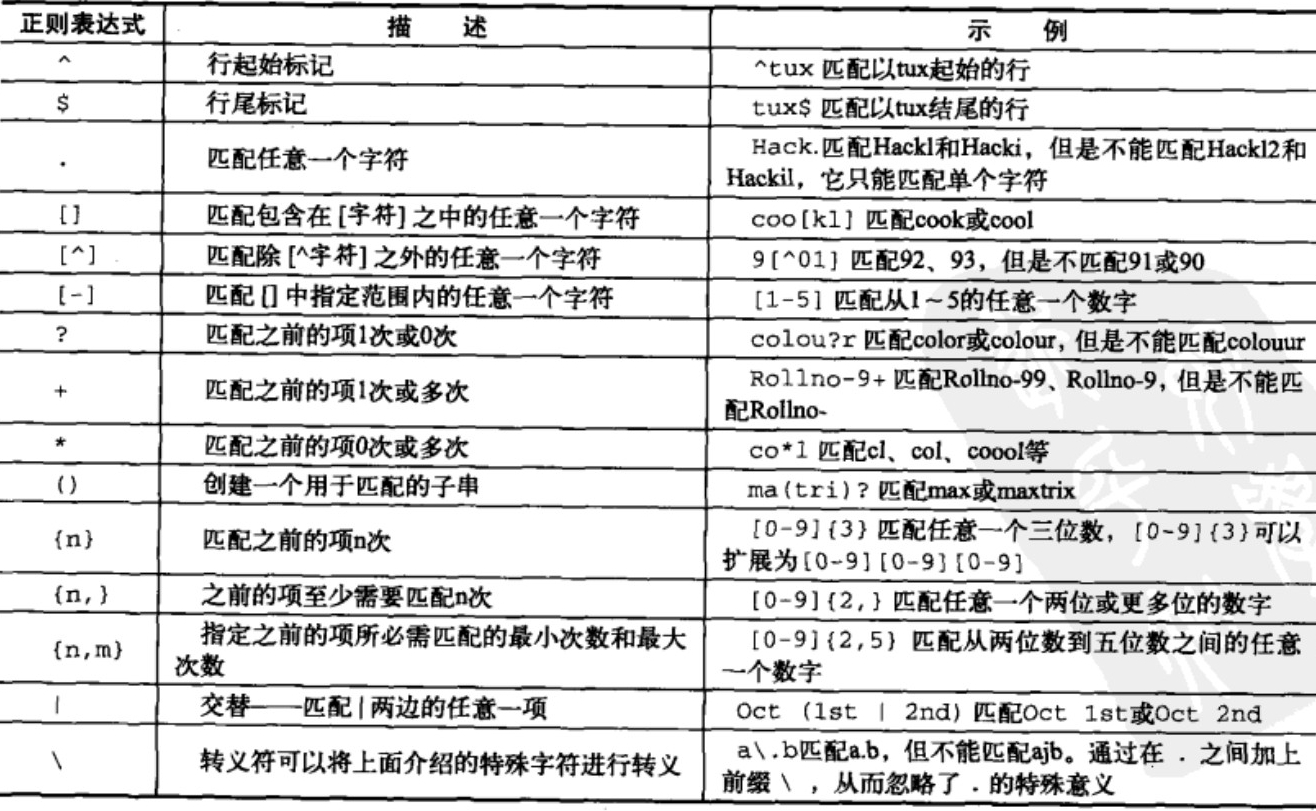
\includegraphics[width=12cm]{c5.meta.03.jpg}
  \end{figure}
\end{frame}

\begin{frame}
  \frametitle{正则和元字符 | 元字符}
  \begin{figure}
    \centering
    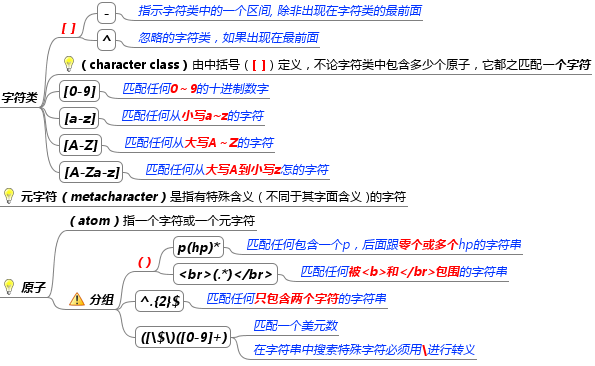
\includegraphics[width=12cm]{c5.re.01.png}
  \end{figure}
\end{frame}

\begin{frame}
  \frametitle{正则和元字符 | 元字符}
  \begin{figure}
    \centering
    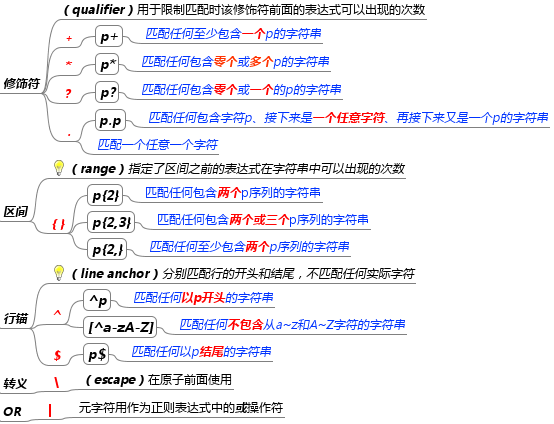
\includegraphics[width=10cm]{c5.re.02.png}
  \end{figure}
\end{frame}

\subsection{正则表达式}
\begin{frame}
  \frametitle{正则和元字符 | 正则表达式 | 元字符}
  \begin{figure}
    \centering
    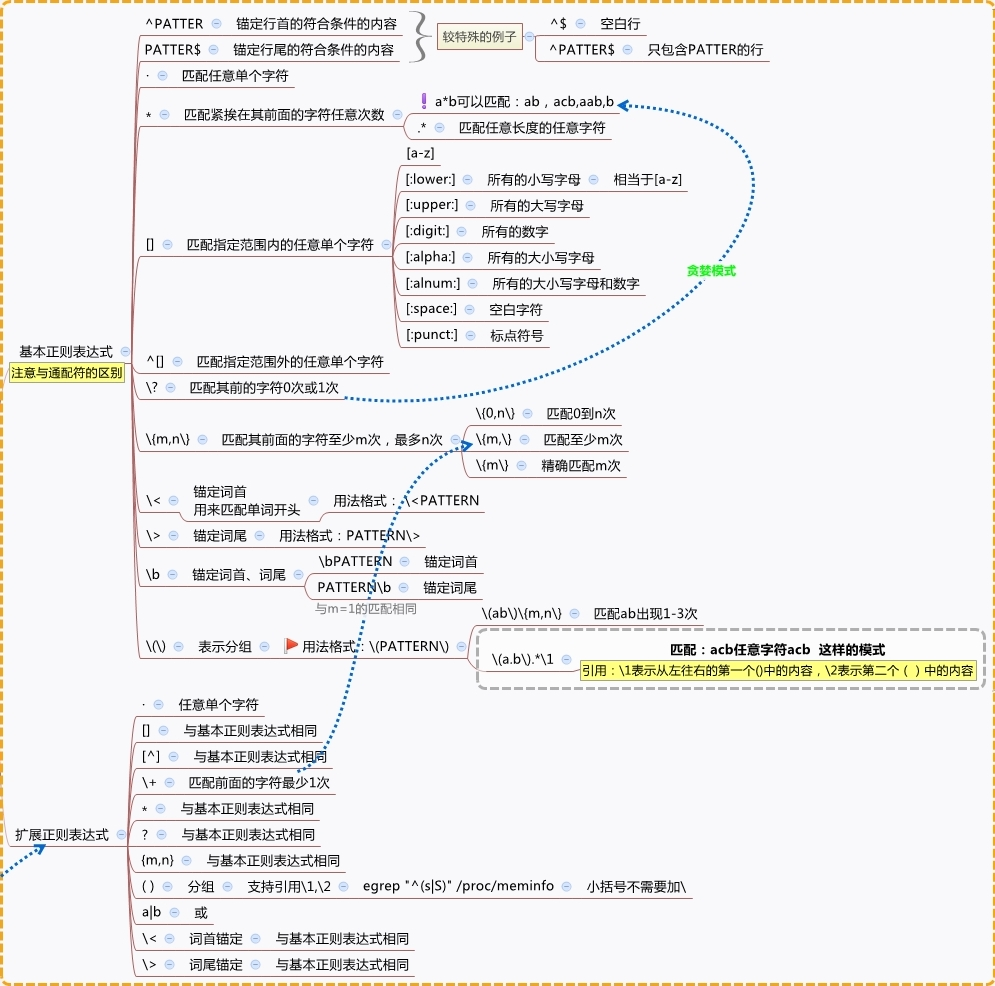
\includegraphics[width=11cm,height=8cm]{c5.re.03.jpg}
  \end{figure}
\end{frame}

\begin{frame}
  \frametitle{正则和元字符 | 正则表达式 | \alert{实例}}
  \begin{figure}
    \centering
    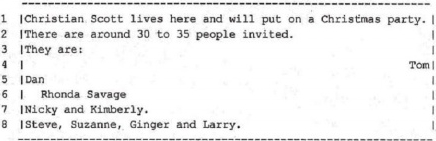
\includegraphics[width=10cm]{c5.re.example.01.jpg}\\
    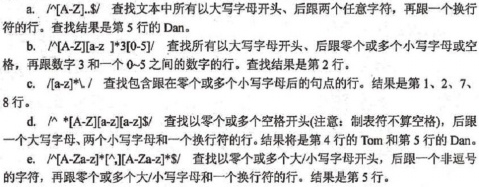
\includegraphics[width=10cm]{c5.re.example.02.jpg}
  \end{figure}
\end{frame}

\begin{frame}[fragile]
  \frametitle{正则和元字符 | 正则表达式 | 复杂实例}
  \begin{block}{正则表达式}
    \begin{itemize}
      \item<2-> \verb|\d+\.\d+\.\d+\.\d+|
      \item<4-> \verb=(^\d{15}$)|(^\d{17}([0-9]|X)$)=
      \item<6-> \verb|^(0[0-9]{2,3}\-)?([2-9][0-9]{6,7})+(\-[0-9]{1,4})?$|
      \item<8-> \verb|/^[a-z]([a-z0-9]*[-_]?[a-z0-9]+)*@([a-z0-9]*[-_]?[a-z0-9]+)+[\.][a-z]{2,3}([\.][a-z]{2})?$/i|
    \end{itemize}
  \end{block}
  \begin{block}{正则含义}
    \begin{itemize}
      \item<3-> IP地址
      \item<5-> 身份证号码(15位或18位)
      \item<7-> 固定电话:3-4位区号,7-8位座机号码,1-4位分机号
      \item<9-> 邮箱地址
    \end{itemize}
  \end{block}
\end{frame}

\begin{frame}[fragile]
  \frametitle{正则和元字符 | 正则表达式 | 易错实例}
  \begin{block}{以下正则表达式中能够抓到abc字符串的有:}
    \begin{enumerate}
      \item \verb|x*|
      \item \verb|ax*|
      \item \verb|abx*|
      \item \verb|ax*b|
      \item \verb|abcx*|
      \item \verb|abx*c|
      \item \verb|ax*bc|
      \item \verb|bx*c|
      \item \verb|bcx*|
      \item \verb|x*bc|
    \end{enumerate}
  \end{block}
\end{frame}

\begin{frame}
  \frametitle{正则和元字符 | 正则表达式 | 比较}
  \begin{itemize}
    \item 在命令行(command line)的位置里,通配符(wildcard)只作用于参数(argument)的路径(path)上
    \item 正则表达式(RE)却只用于"字符串处理" 的程序中,这与路径名一点关系也没有
    \item 正则表达式(RE)所处理的字符串,通常是指纯文本或通过stdin读进的内容
  \end{itemize}
\end{frame}


\section{find和grep}
\subsection{find}
\begin{frame}[fragile]
  \frametitle{find | 选项}
  \begin{table}
    \centering
    \rowcolors[]{1}{blue!20}{blue!10}
    \begin{tabularx}{0.9\textwidth}{cX}
      \hline
      \rowcolor{blue!50}选项 & 说明\\
      \hline
      \verb|--help| & 显示帮助信息\\
      %\verb|--maxdepth n| & 向下搜索到第n层目录\\
      %\verb|--mindepth n| & 至少向下搜索n层子目录\\
      \verb|--maxdepth n| & (最多)向下搜索到第n层子目录\\
      \verb|--mindepth m| & (至少)从第m层子目录开始搜索\\
      \verb|--mount| & 防止搜索其他文件系统\\
      \hline
    \end{tabularx}
  \end{table}
\end{frame}

\begin{frame}
  \frametitle{find | \alert{测试}}
  \begin{table}
    \centering
    \rowcolors[]{1}{blue!20}{blue!10}
    \begin{tabularx}{0.9\textwidth}{cX}
      \hline
      \rowcolor{blue!50}测试 & 说明\\
      \hline
      +n & 搜索大于数字n的所有内容\\
      -n & 搜索小于数字n的所有内容\\
      n & 搜索准确匹配数字n的所有内容\\
      -amin +n & 搜索n分钟之前访问过的文件\\
      -atime -n & 搜索n天内访问过的文件\\
      -fstype TYPE & 搜索指定类型的文件系统\\
      -gid n & 搜索GID等于n的文件\\
      -group GROUP & 搜索组名为GROUP的文件\\
      -name FILE & 搜索名为FILE的文件(可以使用通配符)\\
      -perm MODE & 搜索权限设置为MODE的文件\\
      -size n & \small{搜索大小等于n的文件(可以使用k、M、G等)}\\
      -type TYPE & 搜索TYPE类型的文件(如d、f、l等)\\
      -uid n & 搜索UID为n的文件\\
      -user USER & 搜索用户名为USER的文件\\
      \hline
    \end{tabularx}
  \end{table}
\end{frame}

\begin{frame}
  \frametitle{find | 测试}
  \begin{figure}
    \centering
    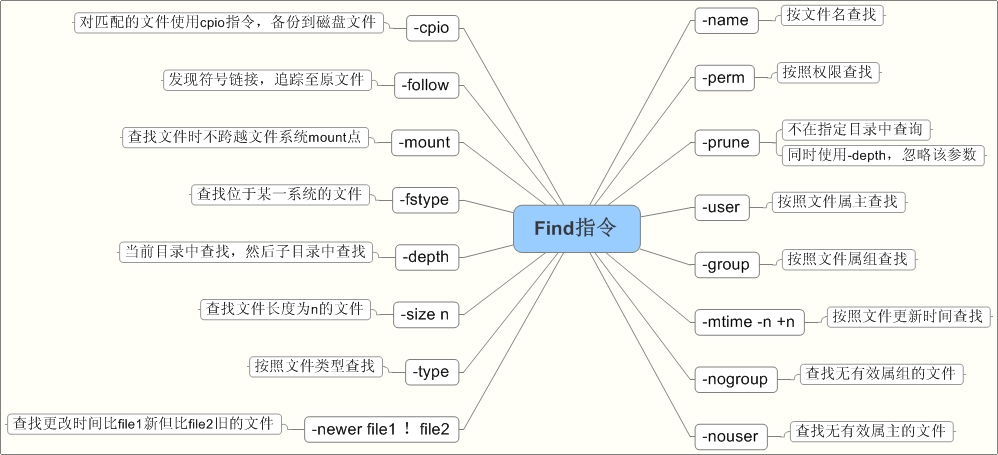
\includegraphics[width=12cm]{c5.find.01.jpg}
  \end{figure}
\end{frame}

\begin{frame}[fragile]
  \frametitle{find | \alert{实例}}
  \begin{block}{实际问题}
    \begin{itemize}
      \item<2-> 找到/etc目录下面的passwd文件
      \item<4-> 找到用户USER在/home目录下拥有的所有文件
      \item<6-> 找到/home目录下大于2G的文件
    \end{itemize}
  \end{block}
  \begin{block}{解决方法}
    \begin{itemize}
      \item<3-> \verb|find /etc -name passwd|
      \item<5-> \verb|find /home -user USER|
      \item<7-> \verb|find /home -size +2G -print|
    \end{itemize}
  \end{block}
\end{frame}

\begin{frame}[fragile]
  \frametitle{find | \alert{实例}}
  \begin{figure}
    \centering
    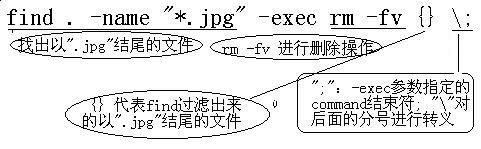
\includegraphics[width=11cm]{c5.find.02.jpg}
  \end{figure}
  \pause
  \begin{block}{\textbackslash; vs. ';' \qquad -exec vs. -ok}
  \begin{itemize}
    \item \verb|find -name "*.swp" -exec rm {} \;|
    \item \verb|find -name "*.swp" -exec rm {} ';'|
    \item \verb|find -name "*.swp" -ok rm {} \;|
  \end{itemize}
  \end{block}
\end{frame}

\subsection{grep}
\begin{frame}[fragile]
  \frametitle{grep | 简介}
  \begin{description}
    \item[定义] Globally search a Regular Expression and Print(全局正则表达式打印)
    \item[功能] 在文件中搜索用户所指定的序列,然后将结果打印出来
    \item[用途] 搜索文件或者在文件中进行查找
    \item[结构] \verb|grep StringToSearchFor FileToSearch|
  \end{description}
\end{frame}

\begin{frame}
  \frametitle{grep | \alert{选项}}
  \begin{figure}
    \centering
    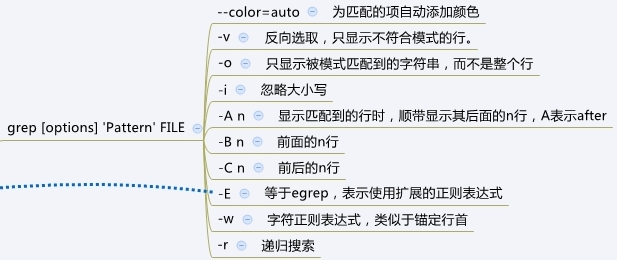
\includegraphics[width=12cm]{c5.grep.01.jpg}
  \end{figure}
\end{frame}

\begin{frame}
  \frametitle{grep | 使用方法}
  \begin{figure}
    \centering
    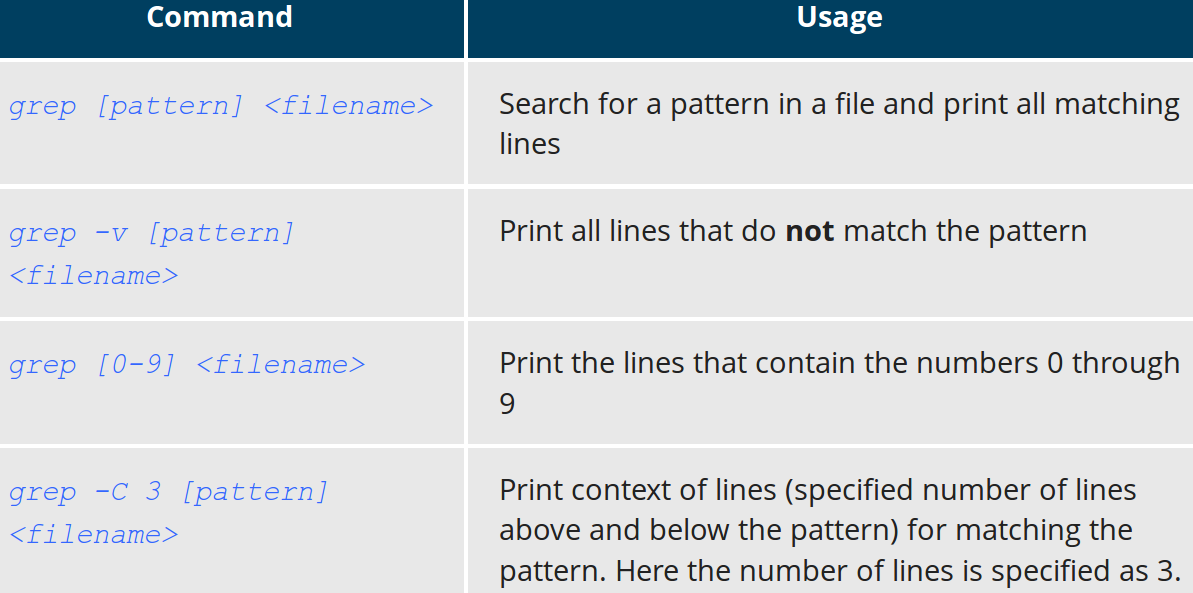
\includegraphics[width=12cm]{c5.grep.10.png}
  \end{figure}
\end{frame}


\begin{frame}[fragile]
  \frametitle{grep | \alert{实例}}
  \begin{block}{实际问题}
    \begin{itemize}
      \item<2-> 在/etc目录下面的文件中搜索root字符串
      \item<4-> 搜索/etc/passwd中不含root字符串的所有账户
      \item<6-> 搜索/etc/passwd中包含root字符串的所有账户
    \end{itemize}
  \end{block}
  \begin{block}{解决方法}
    \begin{itemize}
      \item<3-> \verb|grep root /etc/*|
      \item<5-> \verb|grep -v root /etc/passwd|
      \item<7-> \verb=cat /etc/passwd | grep root=
    \end{itemize}
  \end{block}
\end{frame}

\begin{frame}
  \frametitle{grep | 实例}
  \begin{figure}
    \centering
    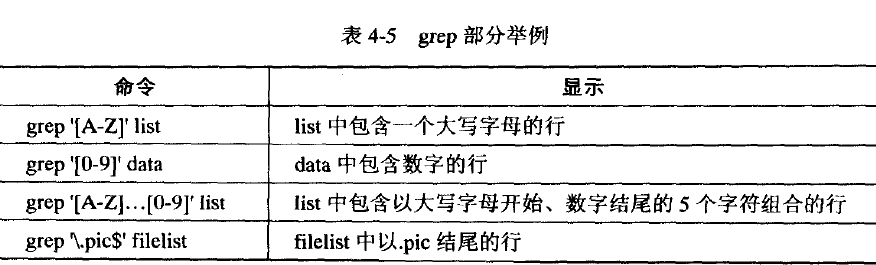
\includegraphics[width=12cm]{c5.grep.02.png}
  \end{figure}
\end{frame}

\begin{frame}[fragile]
  \frametitle{grep | \alert{应用实例}}
  \begin{block}{具体问题}
    \begin{itemize}
      \item<2-> 不区分大小写,查找包括“the”的行,并显示行号
      \item<4-> 查找不包括“the”的行,统计行数
      \item<6-> 查找空白行
      \item<8-> 查找包括2-5个字母o的行
    \end{itemize}
  \end{block}
  \begin{block}{grep命令}
    \begin{itemize}
      \item<3-> \verb|grep -in "the" input.txt|
      \item<5-> \verb|grep -cv "the" input.txt|
      \item<7-> \verb|grep -n "^$" input.txt|
      \item<9-> \verb|grep -n "o\{2,5\}" input.txt|
    \end{itemize}
  \end{block}
\end{frame}

\section{文本处理命令}
\begin{frame}
  \frametitle{\alert{文本处理命令}}
  \begin{figure}
    \centering
    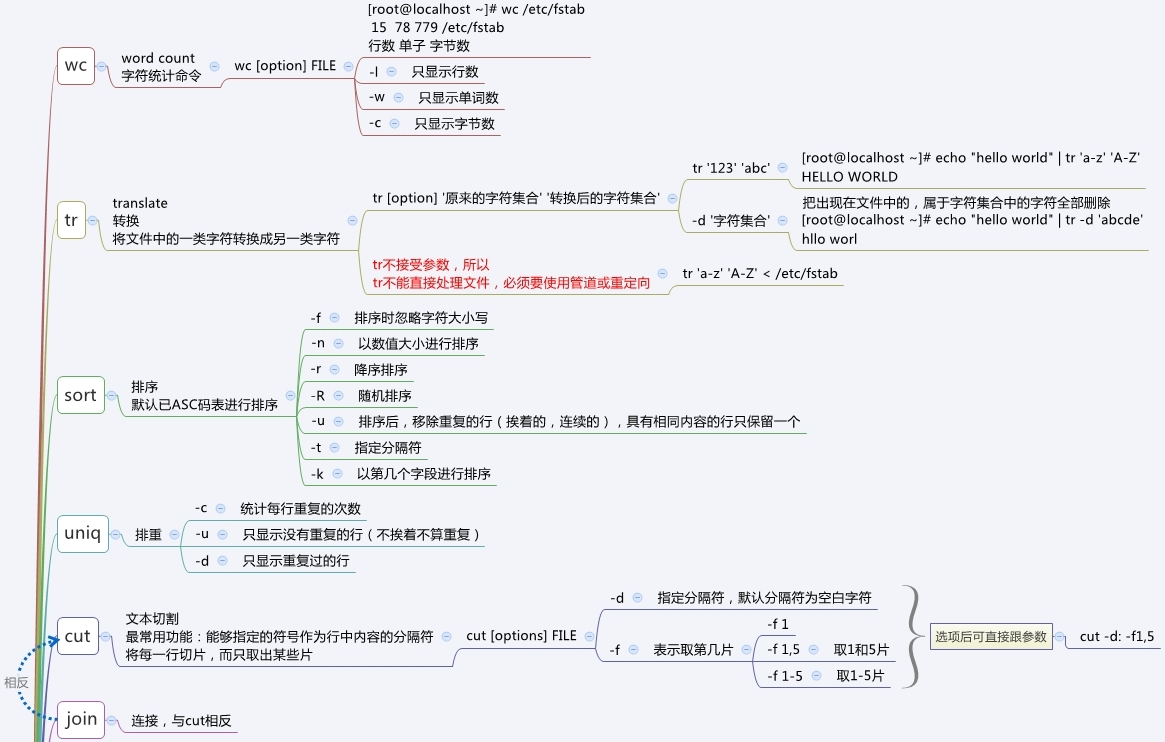
\includegraphics[width=12cm]{c5.text.01.jpg}
  \end{figure}
\end{frame}

\begin{frame}[fragile]
  \frametitle{文本处理命令 | sort}
  \begin{block}{sort}
    \textbf{sort} is used to rearrange the lines of a text file either in ascending or descending order, according to a sort key. You can also sort by particular fields of a file. The default sort key is the order of the ASCII characters (i.e., essentially alphabetically).

    When used with the \verb|-u| option, sort checks for unique values after sorting the records (lines). It is equivalent to running \textbf{uniq} on the output of \textbf{sort}.
  \end{block}
  \pause
  \begin{figure}
    \centering
    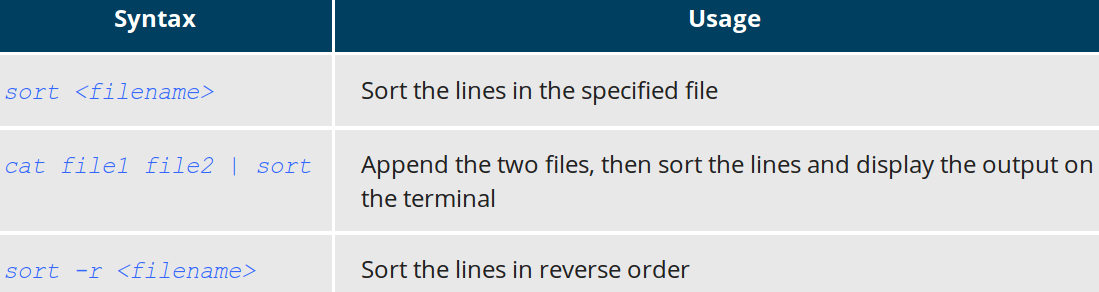
\includegraphics[width=12cm]{c5.sort.01.png}
  \end{figure}
\end{frame}

\begin{frame}[fragile]
  \frametitle{文本处理命令 | uniq}
  \begin{block}{uniq}
    \textbf{uniq} is used to remove duplicate lines in a text file and is useful for simplifying text display. \textbf{uniq} requires that the duplicate entries to be removed are consecutive. Therefore one often runs \textbf{sort} first and then pipes the output into \textbf{uniq}; if sort is passed the \verb|-u| option it can do all this in one step. 

    To remove duplicate entries from some files, use the following command: \verb=sort file1 file2 | uniq > file3=; OR \verb|sort -u file1 file2 > file3|

    To count the number of duplicate entries, use the following command: \verb|uniq -c filename|
  \end{block}
\end{frame}

\begin{frame}[fragile]
  \frametitle{文本处理命令 | paste}
  \begin{figure}
    \centering
    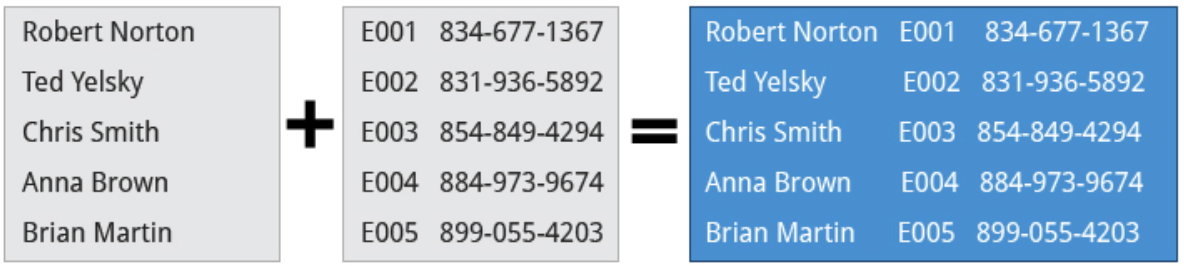
\includegraphics[width=12cm]{c5.paste.01.png}
  \end{figure}
  \pause
  \begin{block}{Commands}
    \begin{itemize}
      \item \verb|paste file1 file2|
      \item \verb|paste -d, file1 file2|
    \end{itemize}
  \end{block}
  \pause
  \begin{block}{Options}
    {\scriptsize
    \begin{itemize}
      \item -d: delimiters, which specify a list of delimiters to be used instead of tabs for separating consecutive values on a single line. Each delimiter is used in turn; when the list has been exhausted, paste begins again at the first delimiter.
      \item -s: which causes \textbf{paste} to append the data in series rather than in parallel; that is, in a horizontal rather than vertical fashion.
    \end{itemize}
    }
  \end{block}
\end{frame}

\begin{frame}[fragile]
  \frametitle{文本处理命令 | join}
  \begin{figure}
    \centering
    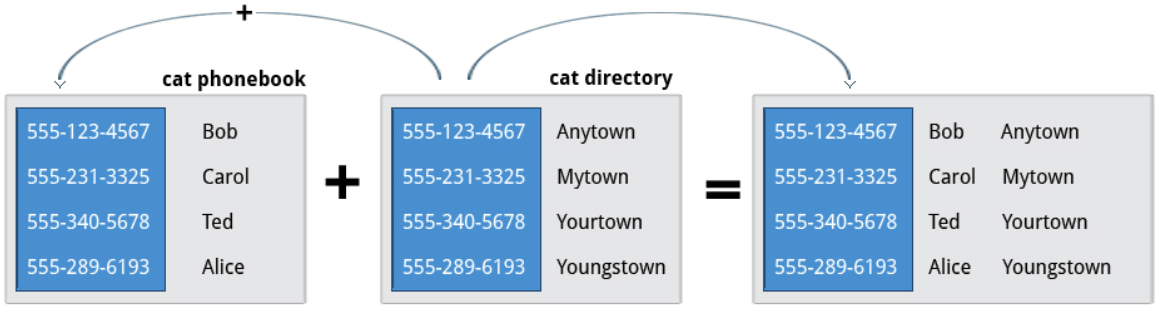
\includegraphics[width=12cm]{c5.join.01.png}
  \end{figure}
  \pause
  \begin{block}{Command}
    \begin{itemize}
      \item \verb|join file1 file2|
    \end{itemize}
  \end{block}
\end{frame}

\begin{frame}[fragile]
  \frametitle{文本处理命令 | split}
  \begin{figure}
    \centering
    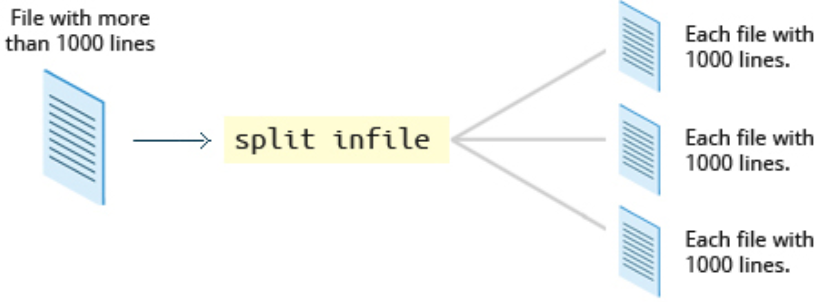
\includegraphics[width=10cm]{c5.split.01.png}
  \end{figure}
  \pause
  \vspace{-0.3cm}
  \begin{block}{Introduction}
    {\footnotesize\textbf{split} is used to break up (or split) a file into equal-sized segments for easier viewing and manipulation, and is generally used only on relatively large files. By default \textbf{split} breaks up a file into 1,000-line segments. The original file remains unchanged, and set of new files with the same name plus an added prefix is created. By default, the \textbf{x} prefix is added. To split a file into segments, use the command \verb|split infile|. To split a file into segments using a different prefix, use the command \verb|split infile <Prefix>|.}
  \end{block}
\end{frame}

\begin{frame}[fragile]
  \frametitle{文本处理命令 | tr}
  The \textbf{tr} utility is used to \textbf{translate} specified characters into other characters or to delete them. The general syntax is as follows: \verb|tr [options] set1 [set2]|\\
  \vspace{0.3cm}
  The items in the square brackets are optional. \textbf{tr} requires at least one argument and accepts a maximum of two. The first, designated \verb|set1| in the example, lists the characters in the text to be replaced or removed. The second, \verb|set2|, lists the characters that are to be substituted for the characters listed in the first argument. Sometimes these sets need to be surrounded by apostrophes (or single-quotes (')) in order to have the shell ignore that they mean something special to the shell. It is usually safe (and may be required) to use the single-quotes around each of the sets.\\
  \vspace{0.3cm}
  To translate all lower case characters to upper case, at the command prompt type \verb=cat filename | tr a-z A-Z =and press the \textbf{Enter} key.
\end{frame}

\begin{frame}
  \frametitle{文本处理命令 | tr}
  \begin{figure}
    \centering
    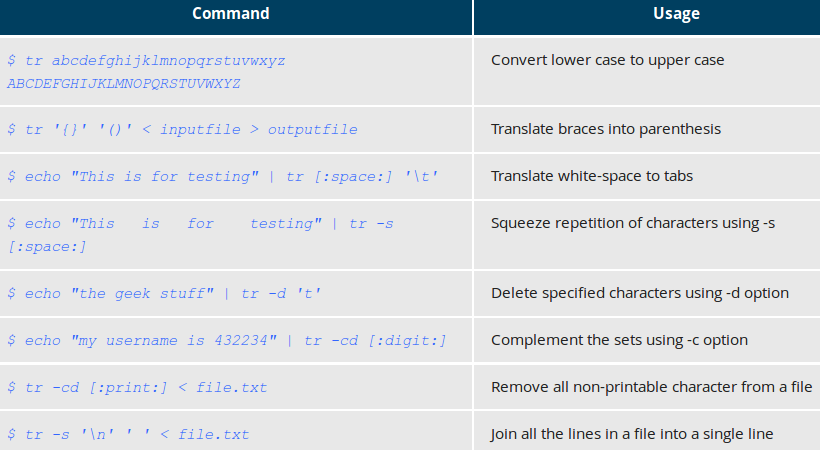
\includegraphics[width=12cm]{c5.tr.01.png}
  \end{figure}
\end{frame}

\begin{frame}[fragile]
  \frametitle{文本处理命令 | tee}
  \textbf{tee} takes the output from any command, and while sending it to standard output, it also saves it to a file. In other words, it "tees" the output stream from the command: one stream is displayed on the standard output and the other is saved to a file.\\
  \vspace{0.3cm}
  For example, to list the contents of a directory on the screen and save the output to a file, at the command prompt type \verb=ls -l | tee newfile= and press the \textbf{Enter} key.
\end{frame}

\begin{frame}[fragile]
  \frametitle{文本处理命令 | wc}
  \textbf{wc} (word count) counts the number of lines, words, and characters in a file or list of files.\\
  \vspace{0.3cm}
  For example, to print the number of lines contained in a file, at the command prompt type \verb|wc -l filename| and press the \textbf{Enter} key.
  \begin{figure}
    \centering
    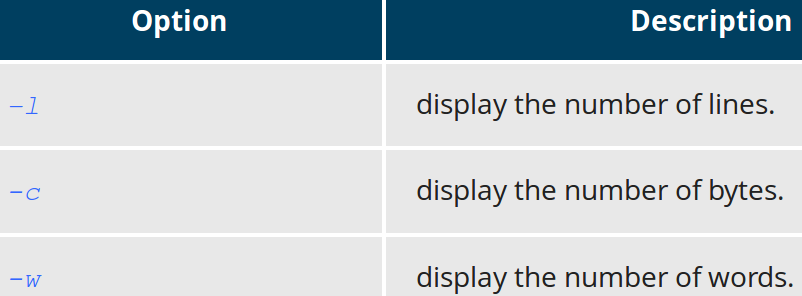
\includegraphics[width=10cm]{c5.wc.01.png}\\
  By default all three of these options are active.
  \end{figure}
\end{frame}

\begin{frame}[fragile]
  \frametitle{文本处理命令 | cut}
  \textbf{cut} is used for manipulating column-based files and is designed to extract specific columns. The default column separator is the \textbf{tab} character. A different delimiter can be given as a command option.\\
  \vspace{0.3cm}
  For example, to display the third column delimited by a blank space, at the command prompt type \verb=ls -l | cut -d" " -f3= and press the \textbf{Enter} key.
\end{frame}

\begin{frame}
  \frametitle{文本处理命令 | less}
  \begin{columns}
    \column{0.7\textwidth}
  Directly opening a large file in an editor will cause issues, due to high memory utilization, as an editor will usually try to read the whole file into memory first. However, one can use \textbf{less} to view the contents of a large file, scrolling up and down page by page without the system having to place the entire file in memory before starting. This is much faster than using a text editor.
    \column{0.3\textwidth}
    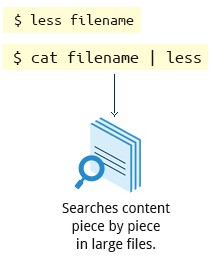
\includegraphics[width=\textwidth]{c5.less.01.jpg}
  \end{columns}
  By default, manual (i.e., the \textbf{man} command) pages are sent through the \textbf{less} command.
\end{frame}

\begin{frame}[fragile]
  \frametitle{文本处理命令 | head}
  \textbf{head} reads the first few lines of each named file (10 by default) and displays it on standard output. You can give a different number of lines in an option.\\
  \vspace{0.3cm}
  For example, If you want to print the first 5 lines from \verb|atmtrans.txt|, use the following command: \verb|head –n 5 atmtrans.txt|. (You can also just say \verb|head -5 atmtrans.txt|.)
\end{frame}

\begin{frame}[fragile]
  \frametitle{文本处理命令 | tail}
  \textbf{tail} prints the last few lines of each named file and displays it on standard output. By default, it displays the last 10 lines. You can give a different number of lines as an option. \textbf{tail} is especially useful when you are troubleshooting any issue using log files as you probably want to see the most recent lines of output.\\
  \vspace{0.3cm}
  For example, to display the last 15 lines of atmtrans.txt, use the following command: \verb|tail -n 15 atmtrans.txt|. (You can also just say \verb|tail -15 atmtrans.txt|.)\\
  \vspace{0.3cm}
  To continually monitor new output in a growing log file: \verb|tail -f atmtrans.txt|. This command will continuously display any new lines of output in atmtrans.txt as soon as they appear. Thus it enables you to monitor any current activity that is being reported and recorded.
\end{frame}

\begin{frame}
  \frametitle{文本处理命令 | nl}
  \begin{block}{nl}
    number lines of files,在文本中插入行号。
  \end{block}
  \pause
  \begin{block}{应用情形}
    \begin{enumerate}
      \item 希望在一些数据中永久插入行号,然后进行保存
      \item 希望在命令的输出中临时插入行号,便于理解
    \end{enumerate}
  \end{block}
  \pause
  \begin{block}{常用选项}
    \begin{itemize}
      \item -v: start,起始号
      \item -i: increment,增量
      \item -b a: body numbering,all lines,对所有行编号
      \item -n: number format,后跟格式代码(ln,rn,rz)
    \end{itemize}
  \end{block}
\end{frame}

\begin{frame}[fragile]
  \frametitle{文本处理命令 | strings}
  \textbf{strings} is used to extract all printable character strings found in
  the file or files given as arguments. It is useful in locating human
  readable content embedded in binary files: for text files one can just
  use \textbf{grep}.\\
  \vspace{0.3cm}
  For example, to search for the string \verb|my_string| in a spreadsheet: \verb=strings book1.xls | grep my_string=.
\end{frame}

\begin{frame}
  \frametitle{文本处理命令 | z Command Family}
  When working with compressed files many standard commands can not be used directly. For many commonly-used file and text manipulation programs there is also a version especially designed to work directly with compressed files. These associated utilities have the letter \textbf{z} prefixed to their name. For example, we have utility programs such as \textbf{zcat}, \textbf{zless}, \textbf{zdiff}, and \textbf{zgrep}.\\
  \begin{figure}
    \centering
    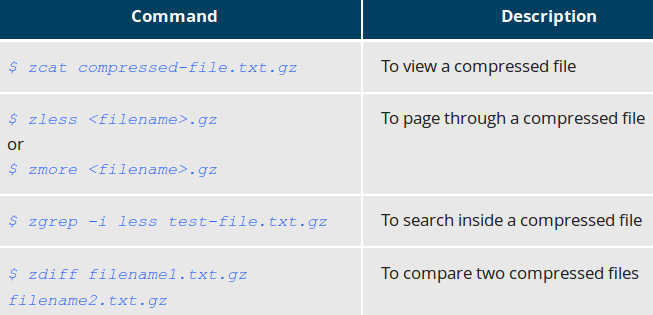
\includegraphics[width=10cm,height=5cm]{c5.z.01.png}
  \end{figure}
\end{frame}

\begin{frame}
  \frametitle{文本处理命令 | z Command Family}
  Note that if you run \textbf{zless} on an uncompressed file, it will still work and ignore the decompression stage. There are also equivalent utility programs for other compression methods besides \textbf{gzip}; i.e, we have \textbf{bzcat} and \textbf{bzless} associated with \textbf{bzip2}, and \textbf{xzcat} and \textbf{xzless} associated with \textbf{xz}.
\end{frame}

\begin{frame}
  \frametitle{文本处理命令 | \alert{实例}}
  \begin{figure}
    \centering
    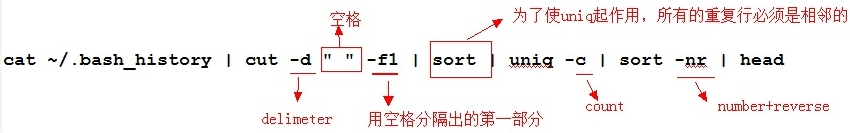
\includegraphics[width=12cm]{c5.text.02.jpg}
  \end{figure}
  \pause
  \begin{block}{解决的问题}
    找出使用频率最高(排名前十位)的命令,并统计其使用次数
  \end{block}
\end{frame}

\begin{frame}
  \frametitle{文本处理命令 | 命令汇总(1/2)}
  \begin{table}
    \centering
    \rowcolors[]{1}{blue!20}{blue!10}
    \begin{tabularx}{\textwidth}{cX|cX}
      \hline
      \rowcolor{blue!50}命令 & 说明 & 命令 & 说明\\
      \hline
      cat & 组合文件 & split & 分割文件\\
      tac & 反转文本行的顺序 & rev & 反转字符串的顺序\\
      head & 从数据开头选择数据行 & tail & 从数据末尾选择数据行\\
      less & 显示文件 & more & 显示文件\\
      colrm & 删除数据列 & cmp & 比较任意两个文件\\
      cut & 抽取数据列/字段 & paste & 组合数据列\\
      nl & 创建行号 & wc & 统计行/单词/字符数量\\
      fold & 格式化行 & fmt & 格式化段落\\
      sort & 排序数据 & uniq & 查找重复行\\
      \hline
    \end{tabularx}
  \end{table}
\end{frame}

\begin{frame}
  \frametitle{文本处理命令 | 命令汇总(2/2)}
  \begin{table}
    \centering
    \rowcolors[]{1}{blue!20}{blue!10}
    \begin{tabularx}{\textwidth}{cX|cX}
      \hline
      \rowcolor{blue!50}命令 & 说明 & 命令 & 说明\\
      \hline
      join & 合并两个文件中的有序数据 & strings & 在二进制文件中搜索字符串\\
      tr & 转换字符 & tsort & 由偏序创建全序\\
      comm & 比较有序文本文件 & diff & 比较无序文本文件\\
      expand & 将制表符转换成空格 & unexpand & 将空格转换成制表符\\
      tee & 管道分流 & pr & 按页/列格式化文本\\
      grep & 选取包含特定模式的行 & look & 查找以特定模式开头的行/单词\\
      sed & 非交互式文本编辑 & awk & 格式化输出\\
      shuf & 随机选取行/文件 & & \\
      \hline
    \end{tabularx}
  \end{table}
\end{frame}

\section{sed和AWK}
\begin{frame}
  \frametitle{sed和AWK | 简介}
  \begin{block}{简单定义}
    \begin{itemize}
      \item sed:处理纯文本流的文本编辑器
      \item AWK:一种输出格式化语言
    \end{itemize}
  \end{block}
  \pause
  \begin{block}{处理对象}
    对已有文本进行操作:
    \begin{itemize}
      \item 管理文件(如/etc/passwd)的内容
      \item 另一个命令(如ls)的输出
      \item 冗长的文本文件(如FASTA格式的序列)的内容
    \end{itemize}
  \end{block}
\end{frame}

\subsection{sed}
\begin{frame}
  \frametitle{sed | 简介}
  \begin{block}{简介}
    sed(Stream EDitor)是一个精简的、非交互式的流编辑器,它根据用户预先设置的规则来操作指定的文本流。
  \end{block}
  \pause
  \begin{block}{工作原理}
    逐行读取文件内容存储在临时缓冲区中,称为“模式空间”(pattern space),接着用sed命令处理缓冲区中的内容,处理完成后,把缓冲区的内容送往屏幕。接着处理下一行,这样不断重复,直到文件末尾。原文件内容并没有改变。
  \end{block}
  \pause
  \begin{block}{\alert{选项}}
    \begin{description}
      \item[-e] Expression,指定多个编辑命令
      \item[-f] File,指定sed命令脚本文件
      \item[-n] 阻止输入行自动输出(只有经过sed处理过的行才显示出来,其他不显示)
    \end{description}
  \end{block}
\end{frame}

\begin{frame}
  \frametitle{sed | 使用方法}
  \begin{figure}
    \centering
    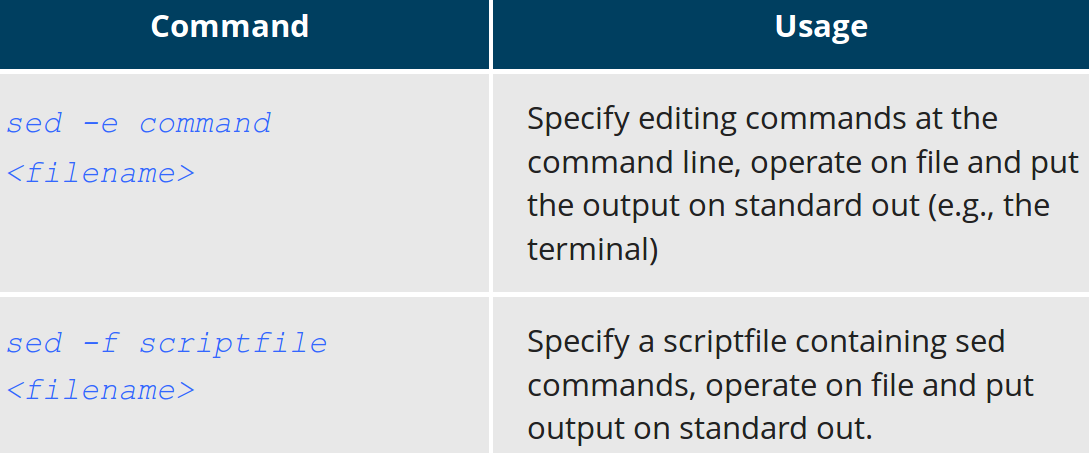
\includegraphics[width=11cm]{c5.sed.20.png}
  \end{figure}
\end{frame}

\begin{frame}[fragile]
  \frametitle{sed | 使用方法 | 替换}
  \begin{figure}
    \centering
    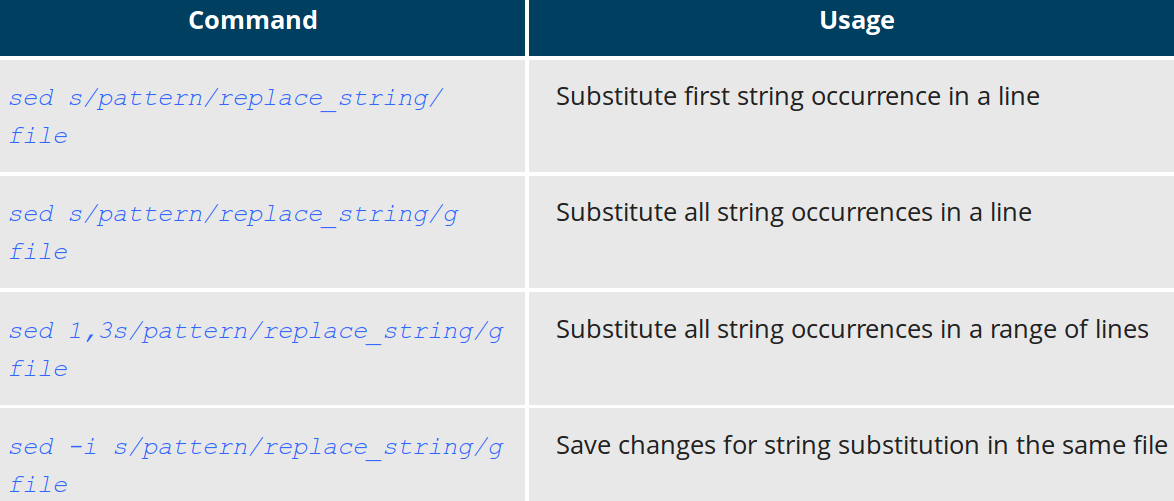
\includegraphics[width=11cm]{c5.sed.sub.01.png}
  \end{figure}
  You must use the \verb|-i| option with care, because the action is not reversible. It is always safer to use \verb|sed| without the \verb|–i| option and then replace the file yourself, as shown in the following example: \\ \verb|sed s/pattern/replace_string/g file > file2|
\end{frame}

\begin{frame}
  \frametitle{sed | 工作原理}
  \begin{figure}
    \centering
    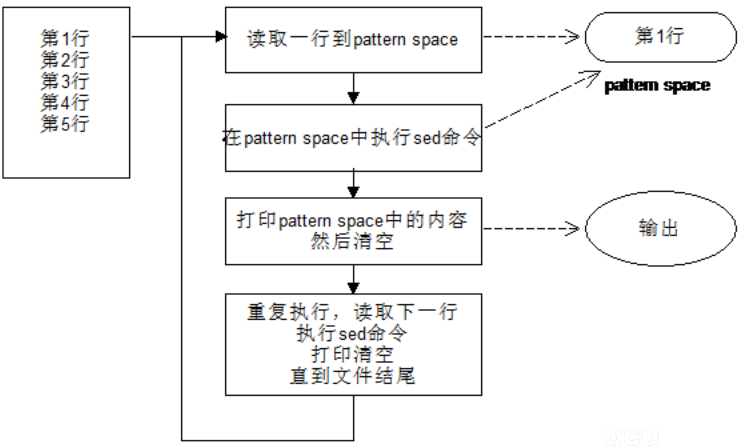
\includegraphics[width=11cm]{c5.sed.step.01.png}
  \end{figure}
\end{frame}

\begin{frame}[fragile]
  \frametitle{sed | \alert{实例}}
  \begin{block}{sed命令}
    \begin{itemize}
      \item<2-> \verb|sed s/Paul/Pablo/g names1.txt > names3.txt|
      \item<4-> \verb|sed 's/Paul/Pablo/g;s/Pat/Patricia/g' names1.txt names2.txt|
      \item<6-> \verb|sed -e 's/Paul/Pablo/g' -e 's/Pat/Patricia/g' names1.txt names2.txt|
      \item<8-> \verb|sed -f edits.sedscr names1.txt > names3.txt|
    \end{itemize}
  \end{block}
  \begin{block}{命令解释}
    \begin{itemize}
      \item<3-> 把Paul替换为Pablo;g表示进行全局查找和替换
      \item<5-> 把Paul和Pat分别替换为Pablo和Patricia
      \item<7-> 效果同上,写法不同
      \item<9-> 根据edits.sedscr文件中的命令进行sed操作
    \end{itemize}
  \end{block}
\end{frame}

\begin{frame}
  \frametitle{sed | 定位}
  \begin{figure}
    \centering
    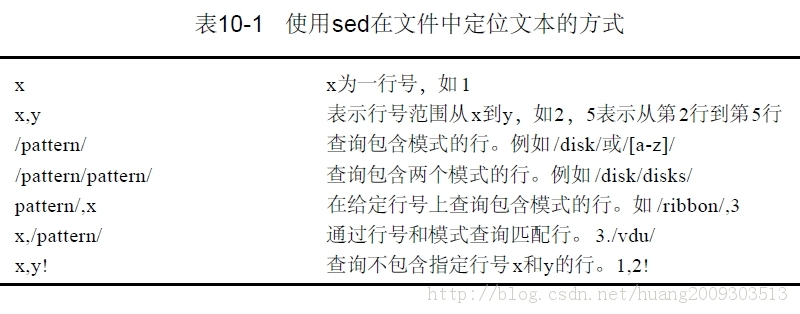
\includegraphics[width=11cm]{c5.sed.line.01.jpg}
  \end{figure}
\end{frame}

\begin{frame}[fragile]
  \frametitle{sed | \alert{定位}}
  \begin{table}
    \centering
    \rowcolors[]{1}{blue!20}{blue!10}
    \begin{tabularx}{\textwidth}{cX}
      \hline
      \rowcolor{blue!50}命令 & 说明\\
      \hline
      \verb|n| & 第n行\\
      \verb|$| & 最后一行\\
      \verb|m,n| & 从第m行到第n行\\
      \verb|/pattern/| & 包含指定模式的行\\
      \verb|/pattern/,n| & 从包含指定模式的行到第n行\\
      \verb|n,/pattern/| & 从第n行到包含指定模式的行\\
      \verb|/pattern1/,/pattern2/| & 从包含模式1的行到包含模式2的行\\
      \verb|!| & 反向选择,不包含指定行,如 \verb|m,n!|\\
      \hline
    \end{tabularx}
  \end{table}
\end{frame}

\begin{frame}
  \frametitle{sed | 命令}
  \begin{figure}
    \centering
    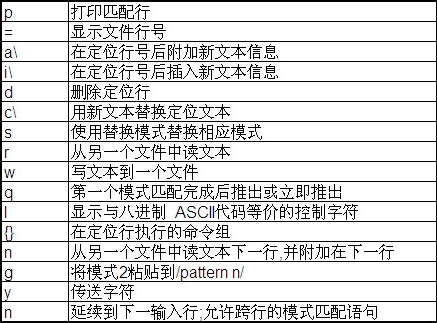
\includegraphics[width=11cm,height=7.5cm]{c5.sed.command.01.jpg}
  \end{figure}
\end{frame}

\begin{frame}[fragile]
  \frametitle{sed | \alert{命令}}
  \begin{table}
    \centering
    \rowcolors[]{1}{blue!20}{blue!10}
    \begin{tabularx}{0.8\textwidth}{ccX}
      \hline
      \rowcolor{blue!50}命令 & 助记 & 说明\\
      \hline
      \verb|p| & Print & 打印匹配行\\
      \verb|=| & --- & 显示匹配行的行号\\
      \verb|d| & Delete & 删除匹配行\\
      \verb|a\ | & Append &  在指定行后面追加文本\\
      \verb|i\ | & Insert & 在指定行后面插入文本\\
      \verb|c\ | & Correct & 用新文本替换指定行\\
      %\verb|c\ | & --- & 用新文本替换指定行\\
      %\verb|s| & --- & 替换命令\\
      \verb|s| & Substitute & 替换命令\\
      \verb|l| & List & 显示指定行中的所有字符\\
      \verb|r| & Read & 读取文件\\
      \verb|w| & Write & 写入文件\\
      %\verb|n| & --- & 读取指定行的下一行\\
      \verb|n| & Next & 读取指定行的下一行\\
      \verb|q| & Quit & 退出sed\\
      \hline
    \end{tabularx}
  \end{table}
\end{frame}

\begin{frame}
  \frametitle{sed | 命令}
  \begin{figure}
    \centering
    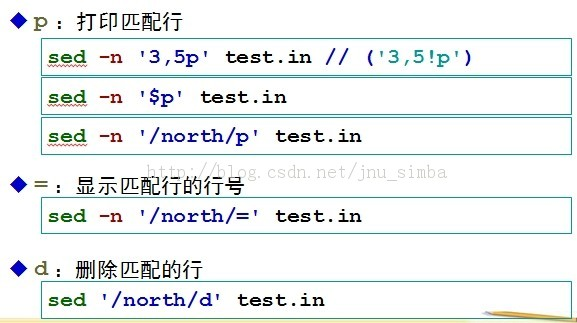
\includegraphics[width=11cm]{c5.sed.command.02.jpg}
  \end{figure}
\end{frame}

\begin{frame}
  \frametitle{sed | 命令}
  \begin{figure}
    \centering
    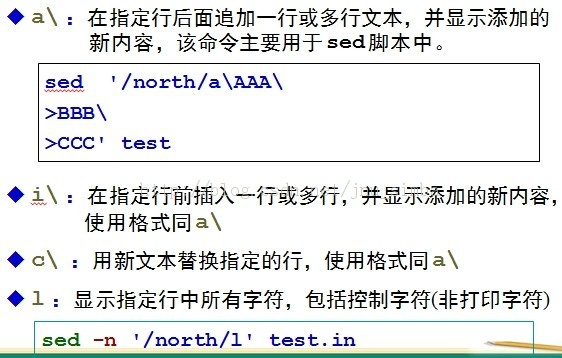
\includegraphics[width=11cm]{c5.sed.command.03.jpg}
  \end{figure}
\end{frame}

\begin{frame}
  \frametitle{sed | 命令}
  \begin{figure}
    \centering
    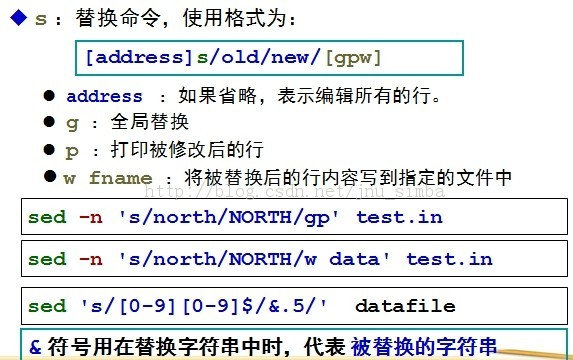
\includegraphics[width=11cm]{c5.sed.command.04.jpg}
  \end{figure}
\end{frame}

\begin{frame}
  \frametitle{sed | 命令}
  \begin{figure}
    \centering
    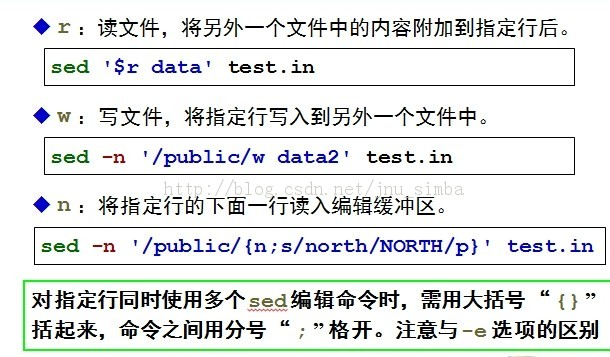
\includegraphics[width=11cm]{c5.sed.command.05.jpg}
  \end{figure}
\end{frame}

\begin{frame}[fragile]
  \frametitle{sed | \alert{应用实例}}
  \begin{block}{具体问题}
    \begin{itemize}
      \item<2-> 输出文件除1-3行之外的行 
      \item<4-> 输出匹配“the”的行,并且输出每行行号
      \item<6-> 将“this”全部替换成“that”
      \item<8-> 添加文件扩展名
      \item<10-> 输出 \verb|ls -l|结果中的第1-3行
    \end{itemize}
  \end{block}
  \begin{block}{sed命令}
    \begin{itemize}
      \item<3-> \verb|sed -n '1,3!p' 123.txt|
      \item<5-> \verb|sed -n -e '/the/p' -e '/the/=' 123.txt|
      \item<7-> \verb|sed 's/this/that/g' 123.txt|
      \item<9-> \verb=echo "hello" | sed 's/$/.txt/g'=
      \item<11-> \verb=ls -l | sed -n '1,3p'=
    \end{itemize}
  \end{block}
\end{frame}

\begin{frame}[fragile]
  \frametitle{sed | 应用实例}
  \begin{block}{To convert 01/02/\ldots \ to JAN/FEB/\ldots}
    \verb|sed -e 's/01/JAN/' -e 's/02/FEB/' -e 's/03/MAR/' \|
    \verb|-e 's/04/APR/' -e 's/05/MAY/' -e 's/06/JUN/' \|
    \verb|-e 's/07/JUL/' -e 's/08/AUG/' -e 's/09/SEP/' \|
    \verb|-e 's/10/OCT/' -e 's/11/NOV/' -e 's/12/DEC/'|
  \end{block}
\end{frame}

\subsection{AWK}
\begin{frame}
  \frametitle{AWK | 简介}
  \begin{block}{简介}
    AWK是用于模式匹配的一种成熟的、结构化的、解释性的编程语言,用于处理数据和生成报告。
  \end{block}
  \pause
  \begin{block}{工作原理}
    AWK逐行扫描输入(可以是文件或管道等),按给定的模式查找出匹配的行,然后对这些行执行AWK命令指定的操作。与sed一样,AWK不会修改输入文件的内容。可以使用重定向将AWK的输出保存到文件中。
  \end{block}
  \pause
  \begin{block}{\alert{选项}}
    \begin{description}
      \item[-F] Field,指定输入记录字段的分隔符,默认使用环境变量IFS的值
      \item[-f] File,指定AWK命令脚本文件
    \end{description}
  \end{block}
\end{frame}

\begin{frame}
  \frametitle{AWK | 简介}
  \begin{block}{Introduction}
    awk is used to extract and then print specific contents of a file and is often used to construct reports. It was created at Bell Labs in the 1970s and derived its name from the last names of its authors: Alfred \textbf{A}ho, Peter \textbf{W}einberger, and Brian \textbf{K}ernighan.
  \end{block}
  \pause
  \begin{block}{Features}
    \begin{itemize}
      \item It is a powerful utility and interpreted programming language.
      \item It is used to manipulate data files, retrieving, and processing text.
      \item It works well with \textbf{fields} (containing a single piece of data, essentially a column) and \textbf{records} (a collection of fields, essentially a line in a file).
    \end{itemize}
  \end{block}
\end{frame}

\begin{frame}[fragile]
  \frametitle{AWK | 使用方法}
  \begin{figure}
    \centering
    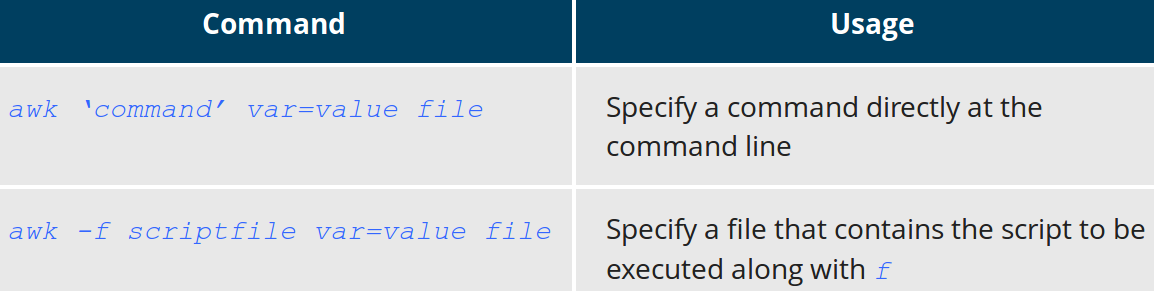
\includegraphics[width=11cm]{c5.awk.20.png}
    \vspace{0.5cm}
    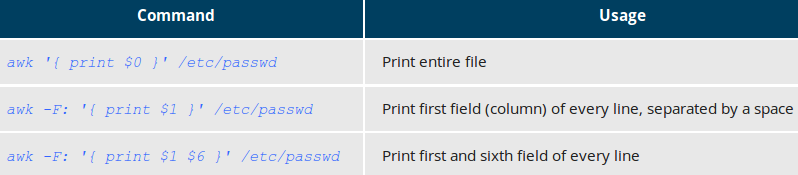
\includegraphics[width=11cm]{c5.awk.print.01.png}
  \end{figure}
\end{frame}

\begin{frame}[fragile]
  \frametitle{AWK | \alert{脚本结构}}
\begin{lstlisting}
awk

  '
  BEGIN {actions}

    /pattern1/{actions}
    ......
    /patternN/{actions}

  END {actions}
  '

InputFile
\end{lstlisting}
\end{frame}

\begin{frame}[fragile]
  \frametitle{AWK | 脚本结构}
  \begin{itemize}
    \item \verb|BEGIN{actions}|和 \verb|END{actions}|是可选的
    \item \verb|/pattern/|和 \verb|{actions}|可以省略,但不能同时省略
      \begin{itemize}
        \item \verb|/pattern/|省略时表示对所有的输入行执行指定的actions
        \item \verb|{actions}|省略时表示打印整行
      \end{itemize}
  \end{itemize}
\end{frame}

\begin{frame}[fragile,label=example]
  \frametitle{AWK | 脚本结构 | 实例}
\begin{lstlisting}
awk

  '
  BEGIN {FS=":"}

  {printf "username: " $1 "\t\t\t user id: " $3}

  END {printf "All done processing /etc/passwd"}
  '

/etc/passwd
\end{lstlisting}
\end{frame}


\begin{frame}
  \frametitle{AWK | \alert{工作原理}}
  \begin{figure}
    \centering
    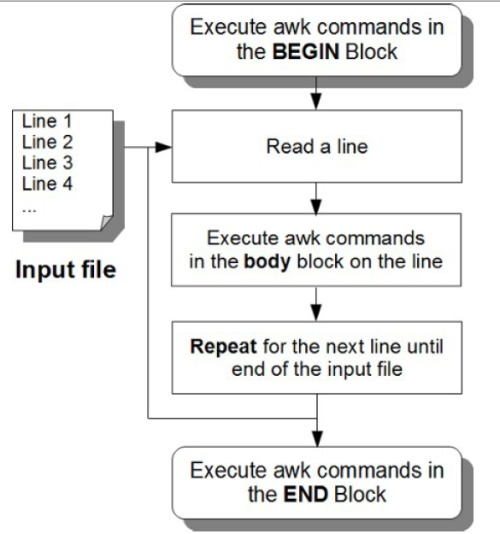
\includegraphics[width=7cm]{c5.awk.step.01.jpg}
  \end{figure}
\end{frame}

\begin{frame}
  \frametitle{AWK | 工作原理}
  \begin{figure}
    \centering
    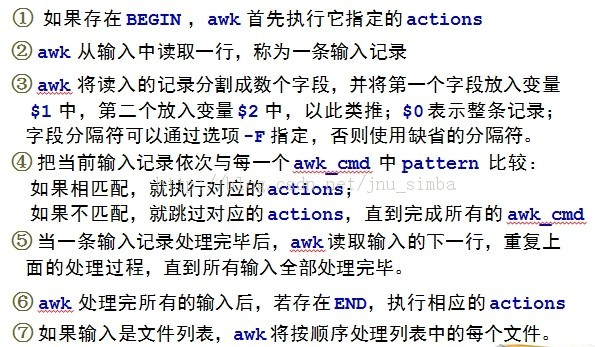
\includegraphics[width=11cm]{c5.awk.step.05.jpg}
  \end{figure}
\end{frame}

\begin{frame}
  \frametitle{AWK | BEGIN | \textcolor{orange}{变量}}
  \begin{figure}
    \centering
    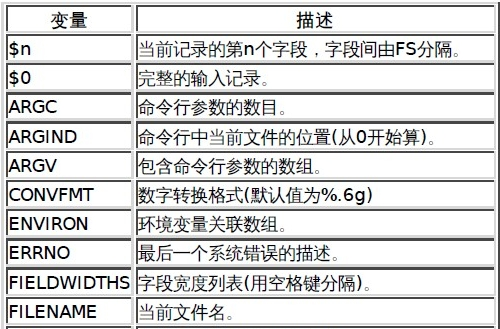
\includegraphics[width=10cm]{c5.awk.01.jpg}
  \end{figure}
\end{frame}

\begin{frame}
  \frametitle{AWK | BEGIN | \textcolor{orange}{变量}}
  \begin{figure}
    \centering
    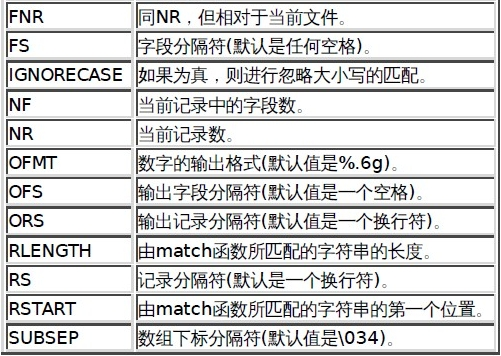
\includegraphics[width=10cm]{c5.awk.02.jpg}
  \end{figure}
\end{frame}

\begin{frame}
  \frametitle{AWK | \alert{命令}}
  \begin{block}{命令构成}
    \begin{enumerate}
      \item 编辑命令(一个、一组命令或一个命令文件)
        \begin{enumerate}
          \item 模式:只编辑与模式相匹配的记录行;没有提供模式时,匹配所有行
          \item 命令:具体执行的编辑命令;没有指定命令时,打印整个记录行
        \end{enumerate}
      \item 要编辑的数据(数据或数据文件)
    \end{enumerate}
  \end{block}
\end{frame}

\begin{frame}
  \frametitle{AWK | 命令 | \alert{记录与字段}}
  \begin{figure}
    \centering
    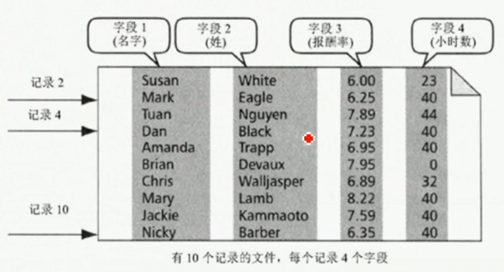
\includegraphics[width=10cm]{c5.awk.03.png}
  \end{figure}
\end{frame}

\begin{frame}
  \frametitle{AWK | 命令 | \alert{记录与字段}}
  \begin{figure}
    \centering
    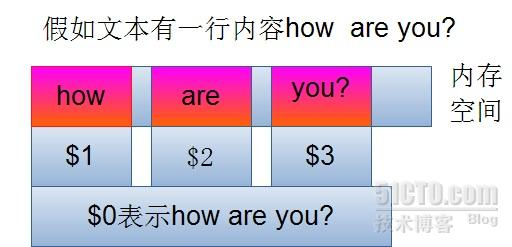
\includegraphics[width=10cm]{c5.awk.04.jpg}
  \end{figure}
\end{frame}

\begin{frame}
  \frametitle{AWK | 命令 | 字段分隔符}
  \begin{figure}
    \centering
    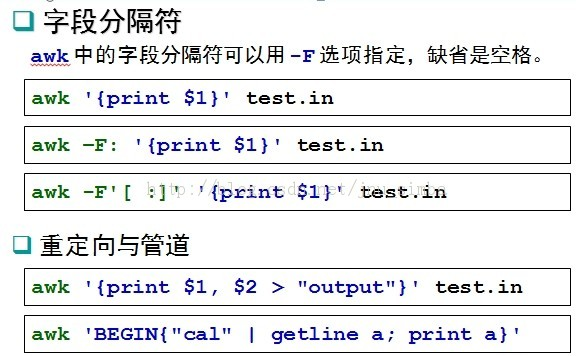
\includegraphics[width=10cm]{c5.awk.cmd.03.jpg}
  \end{figure}
\end{frame}

\begin{frame}
  \frametitle{AWK | 命令 | 表达式}
  \begin{figure}
    \centering
    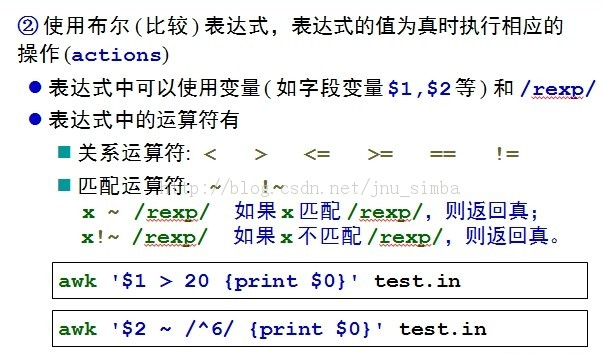
\includegraphics[width=10cm]{c5.awk.cmd.01.jpg}
  \end{figure}
\end{frame}

\begin{frame}
  \frametitle{AWK | 命令 | 表达式}
  \begin{figure}
    \centering
    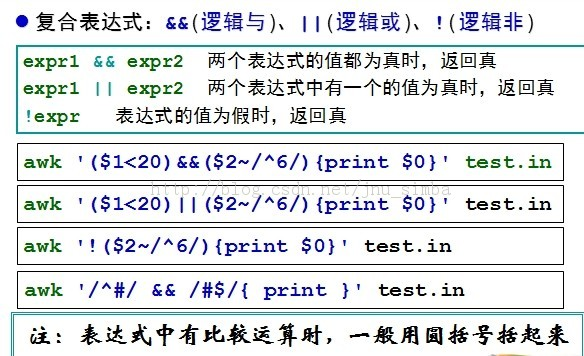
\includegraphics[width=10cm]{c5.awk.cmd.02.jpg}
  \end{figure}
\end{frame}

\begin{frame}[fragile]
  \frametitle{AWK | 命令 | \alert{转义序列}}
  \begin{table}
    \centering
    \rowcolors[]{1}{blue!20}{blue!10}
    \begin{tabularx}{0.8\textwidth}{cX}
      \hline
      \rowcolor{blue!50}转义序列 & 说明\\
      \hline
      \verb|\t| & 制表符,Tab键\\
      \verb|\n| & 换行,新行\\
      \verb|\r| & 回车键\\
      \verb|\'| & 单引号\\
      \verb|\"| & 双引号\\
      \verb|\\| & 反斜线\\
      \verb|\f| & 走纸换页,新页\\
      \verb|\v| & 垂直制表符\\
      \verb|\a| & 警报,警钟\\
      \verb|\b| & 退格键\\
      \hline
    \end{tabularx}
  \end{table}
\end{frame}

\againframe{example}

\begin{frame}[fragile]
  \frametitle{AWK | \alert{应用实例}}
  \begin{block}{具体问题}
    \begin{itemize}
%      \item<2-> 输出文件全部文本
      \item<2-> 输出 \verb|ls -l|中非文件夹的完整信息
      \item<4-> 给文本的每一行添加行号 
      \item<6-> 将文本中的空格换成制表符
      \item<8-> 检测系统中UID为0的用户
      \item<10-> 检测系统中密码为空的用户
    \end{itemize}
  \end{block}
  \begin{block}{命令}
    \begin{itemize}
%      \item<3-> \verb|awk '{print $0}' 123.txt|
      \item<3-> \verb=ls -l | awk '{if($1 !~ /^d/) {print $0}}'=
      \item<5-> {\small \verb|awk '{printf("%03d %s\n",NR,$0)}' ori.txt > dst.txt|}
      \item<7-> \verb|awk 'BEGIN{FS=" ";OFS="\t"} {print $1,$2,$3}' ori.txt > dst.txt|
      \item<9-> \verb|awk -F: '$3==0 {print $1}' /etc/passwd|
      \item<11-> \verb|awk -F: 'length($2)==0 {print $1}' /etc/shadow|
    \end{itemize}
  \end{block}
\end{frame}

\section{生物信息学中的应用}
\begin{frame}[fragile]
  \frametitle{Useful bash one-liners for bioinformatics}
  \begin{block}{具体问题}
    \begin{itemize}
      \item<2-> Count FASTA record
      \item<4-> Split a multi-FASTA file into individual FASTA files
      \item<6-> Convert a FASTQ file to FASTA 
      \item<8-> Returns all lines on Chr 1 between 1MB and 2MB in file.txt 
    \end{itemize}
  \end{block}
  \begin{block}{命令}
    \begin{itemize}
      \item<3-> \verb=grep '>' file.fasta | wc -l=
      \item<5-> \verb|awk '/^>/{s=++d".fa"} {print > s}' multi.fa|
      \item<7-> \verb|sed -n '1~4s/^@/>/p;2~4p' file.fq > file.fa|
      \item<9-> \verb~cat file.txt | awk '$1=="1"' |~ 
	\verb~awk '$3>=1000000' | awk '$3<=2000000'~
    \end{itemize}
  \end{block}
\end{frame}

\begin{frame}[fragile]
  \frametitle{Useful bash one-liners for bioinformatics}
  \begin{block}{具体问题}
    \begin{itemize}
      \item<2-> Print all possible 3mer DNA sequence combinations
      \item<4-> Determine the number of genes annotated in a GFF3 file
      \item<6-> Determine all feature types annotated in a GFF3 file
      \item<8-> Basic FASTQ sequence statistics(number,percentage,\ldots)
    \end{itemize}
  \end{block}
  \begin{block}{命令}
    \begin{itemize}
      \item<3-> \verb=echo {A,C,G,T}{A,C,G,T}{A,C,G,T}=
      \item<5-> \verb|grep -c '\tgene\t' yourannots.gff3|
      \item<7-> \verb~grep -v '^#' GFF3 | cut -s -f 3 | sort | uniq~
      \item<9-> {\tiny \verb~cat myfile.fq | awk '((NR-2)%4==0){read=$1;total++;count[read]++}END{for(read in count){if(!max||count[read]>max) {max=count[read];maxRead=read};if(count[read]==1){unique++}};print total,unique,unique*100/total,maxRead,count[maxRead],count[maxRead]*100/total}'~}
    \end{itemize}
  \end{block}
\end{frame}

\begin{frame}[fragile]
  \frametitle{\alert{Useful bash one-liners for bioinformatics}}
  \begin{block}{具体问题}
    \begin{itemize}
      \item<2-> 基因组中一共有多少基因?
      \item<4-> 获取基因组中所有基因的ID
      \item<6-> 计算每条染色体上的基因数目
      \item<8-> 每条染色体的正负链上各有多少基因?
      \item<10-> 把染色体的正负链按照基因的数目进行排序
    \end{itemize}
  \end{block}
  \begin{block}{命令}
    \begin{itemize}
      \item<3-> \verb=wc -l gene.bed=
      \item<5-> \verb|cut -f4 gene.bed > gene_id.txt|
      \item<7-> \verb=cut -f1 gene.bed | sort | uniq -c=
      \item<9-> \verb=cut -f1,6 gene.bed | sort | uniq -c=
      \item<11-> \verb=cut -f1,6 gene.bed | sort | uniq -c | sort -nr=
    \end{itemize}
  \end{block}
\end{frame}

\begin{frame}
  \frametitle{Linux \& Bioinformatics \& One-Liners}
  \begin{itemize}
    \item \href{http://wiki.bits.vib.be/index.php/Introduction\_to\_Linux\_for\_bioinformatics}{Introduction to Linux for bioinformatics}
    \item \href{http://lh3lh3.users.sourceforge.net/biounix.shtml}{A Bioinformatician's UNIX Toolbox}
    \item \href{http://genomics-array.blogspot.com/2010/11/some-unixperl-oneliners-for.html}{Some unix/perl oneliners for Bioinformatics}
    \item \href{https://wikis.utexas.edu/display/bioiteam/Scott's+list+of+linux+one-liners}{Scott's list of linux one-liners}
    \item \href{https://github.com/stephenturner/oneliners}{Bioinformatics one-liners}
    \item \href{http://www.catonmat.net/series/bash-one-liners-explained}{Article series ``Bash One-Liners Explained"}
    \item \href{http://www.catonmat.net/series/awk-one-liners-explained}{Article series ``Awk One-Liners Explained"}
    \item \href{http://www.catonmat.net/series/sed-one-liners-explained}{Article series ``Sed One-Liners Explained"}
    \item \href{http://www.catonmat.net/series/perl-one-liners-explained}{Article series ``Perl One-Liners Explained"}
    \item \href{http://www.catonmat.net/series/commandlinefu-one-liners-explained}{Article series ``CommandLineFu One-Liners Explained"}
  \end{itemize}
\end{frame}

\section{回顾与总结}
\subsection{总结}
\begin{frame}
  \frametitle{高级工具 | 总结}
  \begin{block}{知识点}
    \begin{itemize}
      \item 元字符(字符,字符集,量词,边界),正则表达式(解析,构建)
      \item find和grep:常用选项,常用测试
      \item 文本处理命令:cut,wc,sort,uniq,\ldots
      \item sed:工作原理,定位方式,编辑命令
      \item AWK:脚本结构,工作原理,常见变量,记录,字段
    \end{itemize}
  \end{block}
  \begin{block}{技能}
    \begin{itemize}
      \item 解析并编写正则表达式
      \item find和grep的基本用法
      \item 文本处理命令的日常使用
      \item 使用sed和AWK处理文本
      \item 正则表达式在grep、sed和AWK中的应用
    \end{itemize}
  \end{block}
\end{frame}

\subsection{思考题}
\begin{frame}
  \frametitle{高级工具 | 思考题}
  \begin{enumerate}
    \item 列举五个常见的元字符并解释其含义。
    \item 根据要求编写正则表达式。
    \item 根据要求使用find查找文件。
    \item 根据要求使用grep查找字符串。
    \item 根据要求组合使用文本处理命令。
    \item 根据要求编写sed脚本编辑文件。
    \item 根据要求编写AWK脚本输出特定字段。
  \end{enumerate}
\end{frame}

\begin{frame}
  \frametitle{下节预告}
   在Windows系统下,你是如何安装、维护软件的?\\
   回顾总结XX软件管家的主要作用,你经常进行的操作。
\end{frame}



\section*{Acknowledgements}
\begin{frame}
  \frametitle{Powered by}
  \begin{center}
    
\includegraphics[width=9cm]{power.png}
  \end{center}
\end{frame}

\end{document}



